% ---------------------------------------------------------------------------
% Author guideline and sample document for EG publication using LaTeX2e input
% D.Fellner, v1.11, Feb 28, 2005

\documentclass{egpubl}
\usepackage{SBIM07}

% --- for  Annual CONFERENCE
% \ConferenceSubmission % uncomment for Conference submission
% \ConferencePaper      % uncomment for (final) Conference Paper
% \STAR                 % uncomment for STAR contribution
% \Tutorial             % uncomment for Tutorial contribution
% \ShortPresentation    % uncomment for (final) Short Conference Presentation
%
% --- for  CGF Journal
% \JournalSubmission    % uncomment for submission to Computer Graphics Forum
% \JournalPaper         % uncomment for final version of Journal Paper
%
% --- for  EG Workshop Proceedings
% \WsSubmission    % uncomment for submission to EG Workshop
 \WsPaper         % uncomment for final version of EG Workshop contribution
%
 \electronicVersion % uncomment if producing the printed version

% for including postscript figures
% mind: package option 'draft' will replace PS figure by a filename within a frame
\ifpdf \usepackage[pdftex]{graphicx} \pdfcompresslevel=9
\else \usepackage[dvips]{graphicx} \fi

\PrintedOrElectronic

% prepare for electronic version of your document
\usepackage{t1enc,dfadobe}

\usepackage{egweblnk}
\usepackage{cite}
\usepackage{verbatim} 
\usepackage{subfigure}

% For backwards compatibility to old LaTeX type font selection.
% Uncomment if your document adheres to LaTeX2e recommendations.
\let\rm=\rmfamily    \let\sf=\sffamily    \let\tt=\ttfamily
\let\it=\itshape     \let\sl=\slshape     \let\sc=\scshape
\let\bf=\bfseries

% end of prologue





% ---------------------------------------------------------------------
% EG author guidelines plus sample file for EG publication using LaTeX2e input
% D.Fellner, v1.12, Oct 21, 2005

\title[Designing a Sketch Recognition Front-End]
      {Designing a Sketch Recognition Front-End: User Perception of
Interface Elements}
%\title[Iterative Design of a Sketch-Based Tool for Pedagogical Circuit Design]%
%      {Iterative Design of a Sketch-Based Tool for Pedagogical Circuit Design}

% for anonymous conference submission please enter your SUBMISSION ID
% instead of the author's name (and leave the affiliation blank) !!
\author[P. Wais, A. Wolin, and C. Alvarado]
       {Paul Wais, Aaron Wolin, and Christine Alvarado
%        S. Spencer$^2$\thanks{Chairman Siggraph Publications Board}
        \\
         Department of Computer Science, Harvey Mudd College,
         Claremont, CA\\
	 \{pwais,awolin,alvarado\}@cs.hmc.edu\\
%        $^2$ Another Department to illustrate the use in papers from authors
%             with different affiliations
       }

% Example
%\author[D. Fellner \& S. Behnke]
%       {D.\,W. Fellner\thanks{Chairman Eurographics Publications Board}$^{1,2}$
%        and S. Behnke$^{2}$
%        S. Spencer$^2$\thanks{Chairman Siggraph Publications Board}
%        \\
%         $^1$TU Darmstadt \& Fraunhofer IGD, Germany\\
%         $^2$Institut f{\"u}r ComputerGraphik \& Wissensvisualisierung, TU Graz, Austria
%        $^2$ Another Department to illustrate the use in papers from authors
%             with different affiliations
%       }
% ------------------------------------------------------------------------

% if the Editors-in-Chief have given you the data, you may uncomment
% the following five lines and insert it here
%
% \volume{23}   % the volume in which the issue will be published;
% \issue{2}     % the issue number of the publication
% \pStartPage{201}      % set starting page


%-------------------------------------------------------------------------
\begin{document}

\maketitle

\begin{abstract}
   Programs that can recognize students' hand-drawn diagrams have the
   potential to revolutionize education by breaking down the barriers
   between diagram creation and simulation.  Much recent work focuses
   on building robust recognition engines, but understanding how to
   support this new interaction paradigm from a user's perspective is
   an equally important and less well understood problem.  We
   present a user study that investigates four critical sketch
   recognition user interface issues: how users integrate the process
   of triggering recognition into their work, when users prefer to
   indicate which portions of the diagram should be recognized, how
   users prefer to receive recognition feedback, and how users
   perceive recognition errors.  We find that user preferences
   emphasize the importance of system reliability, the minimization of
   distractions, and the maximization of predictability. 
   
% Contribution: This paper presents the first direct comparison of critical
%  free-sketch recognition user interface mechanisms through the novel
%  application of a Wizard of Oz evaluation methodology.  We present
%  recommendation for developers of sketch recognition user interfaces 
%  as well as an interface for a sketch recognition digital design tool 
%  informed by our results.


% Benefit: The results of our study directly inform key aspects of
%   sketch recognition user interface design (e.g., how to allow users
%   to trigger recognition and how to provide recognition feedback),
%   and recognition algorithm development (e.g., which types of errors
%   to try to avoid). 

% Research areas:
%  Evaluation
%  Pen UIs
%  Recognition of sketches, diagrams... etc.

% For additional keywords I would list:
% Wizard of Oz Study

 

% results:
% users want reliability of button trigger over convenience of gesture
% users want pre-separation over post separation and want seperation tool to require least work
% users want most efficient interface possible
% users want least invasive feedback; feedback that provides most natural transformation
% users want most predictible errors
% users all use more or less the same approach to using our tool


\begin{classification} % according to http://www.acm.org/class/1998/
\CCScat{H.5.2}{Information Interfaces and Presentation}{User Interfaces}: \textit{Evaluation/methodology, Interaction styles, Prototyping, User-centered design}
\end{classification}

\begin{classification} % according to http://www.acm.org/class/1998/
\CCScat{I.5.4}{Computing Methodologies}{Pattern Recognition}: \textit{Applications}
\end{classification}

%\begin{classification} % according to http://www.acm.org/class/1998/
%\CCScat{J.6}{Computer-Aided Engineering}{Computer-aided design}
%\end{classification}

%\begin{classification} % according to http://www.acm.org/class/1998/
%\CCScat{I.3.3}{Computer Graphics}{Line and Curve Generation}
%\end{classification}

%\begin{classification} % according to http://www.acm.org/class/1998/
%\CCScat{H.1.2}{User/Machine Systems}{Human information processing}
%\end{classification}

\end{abstract}


%-------------------------------------------------------------------------
\section{Introduction}

% example of frustration: += thomas "adapt correct behavior to work for it" is a problem
% intro += crossY CrossY \cite{1029635}
Many engineering classes rely on simulation technologies to help
students understand the systems they design.  Unfortunately, mouse and
keyboard interfaces to these programs are cumbersome.  Students in
these courses draw countless diagrams on paper (or on a Tablet PC)
because sketch-based diagram creation is quicker and more natural.  
In fact, many instructors require students to draw 
diagrams on paper before entering designs into simulation software so
that students focus on their design, not on the software interface.

Systems that can recognize and simulate students' hand-drawn sketches
have the potential to lower the cognitive barrier between students and
simulation software.  However, these systems face their own interface
challenges.

One challenge is how to allow users to trigger recognition and how to
display recognition feedback.  Feedback can be distracting in the
early stages of design \cite{Hong2002Sketch}, but it can also aid
recognition as it can help users adapt their drawing styles to match
the system's expectations.  Researchers have evaluated the usability
of various recognition triggers and feedback mechanisms in isolation
(e.g.,
\cite{Alvarado2001Preserving,Newman2003Denim,LaViola2006Initial}), but
have not compared different techniques directly.

A second challenge is how to allow users to indicate which pieces
of the diagram the system should attempt to recognize.  Students'
homework often consists of a mix of text, equations, and
diagrams. Despite advances in parsing heterogeneous
notes~\cite{Wang2006Parsing}, a recognition system must receive only a
single type of input to be practical.  Most recognition systems allow
the user to draw only one type of input (e.g., electrical
circuits~\cite{Gennari2005Combining}), while a few systems allow the
user to manually select pieces of their drawing to be recognized after
they have finished drawing~\cite{LaViola2006Initial}.  Again, little
is known about which interface users prefer.

A third challenge is to minimize the impact of recognition errors on
usability.  Some systems reduce errors by placing constraints on
users' drawing style.  Others focus on intuitive error correction
mechanisms as a way of reducing the impact of recognition
errors~\cite{Mankoff2000Providing}.  We believe that understanding
users' tolerance for different types of recognition errors can help
guide sketch recognition research by allowing researchers to focus on
eliminating errors that have the biggest impact on usability.  Little
work has been done in this area.

%Richard Davis' SketchWizard (ref SketchWizard) takes the first stride towards constructing a generic, multi-domain tool for %conducting Wizard-of-Oz-based development of sketch-based systems.  Our technique entails the mobilization of SketchWizard's %Wizard of Oz paradigm while simultaneously engineering a Tablet PC application front-end that could potentially wrap future %sketch-recognition engines for further user studies.  


%  through the novel
%application of a Wizard of Oz evaluation methodology.  We present
%  an interface for a sketch recognition digital design tool 
%  informed by our results.
  
To address the above challenges, we present the first direct
comparison of critical free-sketch recognition user interface (UI)
elements.  Unlike prior research, which usually involves a qualitative
analysis of a complete solution, we compare interface elements
directly using a novel application of a Wizard of Oz evaluation
methodology.  Specifically, we evaluate UI mechanisms for triggering
recognition, providing feedback, and separating recognizable from
unrecognized data, and we examine users' perception of different types
of recognition errors.  Our results indicate that:
\begin{itemize}
\item Users prefer to trigger recognition after they are done drawing,
  even when the system produces errors.
\item Users prefer to segregate pieces of the drawing (e.g., diagram
  vs. annotation) at creation time rather than recognition time.
\item Users want recognition feedback to transform and clutter their
  sketch as little as possible (even when they have completely finished sketching).
\item Users prefer errors that are predictable.
\end{itemize}


%% Our study addresses the following questions:
%% \begin{itemize}
%% \item How do users integrate the task of triggering recognition into
%% their workflows?  How can the design of a user interface assist in
%% this integration?
%% \item How do users react to and interpret recognition results?  
%% \item How and when do users perfer to indicate which pieces of the
%%   diagram should be recognized? 
%% \item How do recognition errors effect the user experience? 
%% \item In the domain of digital circuit design, what characteristics of
%% a sketch-based system do users find most desirable?
%% \end{itemize}

One important user interface question that we do not address is how
gesture-based or menu-based interfaces compare to free-sketch
recognition interfaces.  For example, users might prefer a reliable
gesture-based system to an error-prone free-sketch recognition system.
Although this question is important, we focus only on free-sketch
recognition interfaces for two reasons.  First, the students we talked
to expressed a strong desire for a system that could simply transform
diagrams they already produce for coursework into recognized circuit schematics;
they did not want to have to learn a whole new language for
interacting with the simulation software.  Second, we cannot compare
free-sketch recognition systems to gesture or menu-based systems until
we better understand how to design an effective user interface for
these systems.

%% Our study was conducted in a single domain (digital circuit design)
%% and so directly informs the design of a sketch recognition interface
%% for digital circuit design.  However, we believe these preferences may
%% apply to other domains.  \emph{Need a stronger sentence here.}


%-------------------------------------------------------------------------
\section{Related Work}

Previous user studies of sketch-based user interfaces focus mainly on
the development or evaluation of complete systems.  Researchers rely
heavily on interviews and ethnographic studies to identify and understand
user preferences of sketch-based computer tools.  For example,
Landay and Myers designed SILK~\cite{landay95SILK}, a sketch-based
system for user interface design, based on the results of a survey of
professional user interface developers.  Newman \textit{et al.} worked
closely with designers throughout the design of
DENIM~\cite{Newman2003Denim}, a sketch-based system for web page
design.  Their interaction with users revealed that web page
development requires very little sketch recognition: DENIM uses
gesture recognition techniques to recognize pages (rectangles) and
links (arrows) but leaves the rest of the user's sketch unrecognized.
Educational software, on the other hand, requires a deeper
understanding of the user's sketch.  Nevertheless, we rely on the
model these studies provide for how to evaluate sketch-based user
interfaces.

Evaluation of many recognition-intensive systems tends to focus on
recognition error rates, and provides only general insight into user
interface issues (e.g., ``users found recognition errors
frustrating'')~\cite{Alvarado2001Preserving,Gennari2005Combining,Hammond2002Tahuti}.
A few researchers, however, have examined system usability in more
detail.  LaViola's evaluation of MathPad$^{2}$, a sketch-based system
that recognizes freely-drawn equations and physical diagrams, reveals
specific user preferences: users like MathPad$^{2}$'s scribble erase
gesture and find recognition errors frustrating but tolerable for this
task~\cite{LaViola2006Initial}.  Other studies of recognition-based
user interfaces are currently
underway~\cite{Koile2007Supporting,Tenneson2005ChemPad}.  None of
these evaluations directly compare interface elements because of the
difficulty in modifying complete recognition systems.

%% Our Wizard of Oz
%% methogology allows us to simulate a complete recognition system so
%% that we can easily modify user interface elements and determine user
%% preferences for specific interface elements rather than assess the
%% suitability of a completed system for its domain.


Other researchers have studied the usability of pen-based interaction
techniques that are complementary to sketch recognition.  The CrossY
interface~\cite{Apitz04CrossY} explores several novel interface
elements that combine gestures and traditional graphical user
interface components.  Long \textit{et
al.}~\cite{Long00VisualSimilarity} provide a model for measuring the
visual similarity of gestures in an effort to inform effective
gesture design.  Finally Lank and Saund present a model of users'
pen-based selection gestures to inform the design of a faster, more
accurate selection mechanism \cite{Lank2005Sloppy}.  The results of
these previous studies are complementary to our results in the
creation of a complete sketch recognition system.

Finally, though little is known about how free sketch recognition
errors affect usability, researchers have studied user perception of
handwriting and speech recognition errors.  Rhyne and Wolf present
early work in this area~\cite{Rhyne1993Recognition}.  More recently,
Frankish \textit{et al.} find that the relationship between error
rates and user acceptance is dependent on the perceived cost to
benefit ratio of a specific task~\cite{Frankish95RecogAccuracy}.  We
expect that the same trend holds for sketch recognition systems.  Wu
\textit{et al.}  find that handwriting task completion time is most
sensitive to error rates above 6\%~\cite{Wu03ChineseCharacterRecog}.
Munteanu \textit{et al.} find a linear relationship between speech
recognition accuracy and the quality of user experience with
webcasts~\cite{Munteanu2006Effect}.  Although we do not examine error
rates specifically, our analysis helps inform user perception of
sketch recognition errors.

\vspace{-0.02in}

\section{User Interface Elements}
This section describes the interface elements and error types we
compared.  We chose a subset of elements used in existing 
sketch recognition applications and suggested by six pre-study 
participants that provides a restricted yet representative range 
of options.

%\subsection{Recognition Triggers}
We compared three different methods for triggering recognition:
button, gesture and pause.

\begin{itemize}
\item \textbf{Button Trigger.}  The user triggers
recognition by tapping on a large interface button.  This 
option is reminiscent of traditional recognition systems.  
\item \textbf{Gesture Trigger.}  The user triggers
recognition using a ``check-tap'' gesture (a
check mark followed by a dot).  We selected this element because
many systems posit the efficiency and naturalness of gestures over 
GUI widgets.  Furthermore, this particular gesture seemed to be 
reliably recognized in informal tests, is not easily 
confused with diagram-relevant symbols,
and is similar to the ``circle-tap'' gesture used in
MathPad$^2$~\cite{LaViola2006Initial}.  
\item \textbf{Automatic Trigger.}  The system triggers recognition
automatically after a brief pause (4 seconds) in sketching.  We chose
a 4 second pause to accommodate different student work paces.
\end{itemize}

%%   We conjectured that system-triggered
%% recognition may entice users to engage in a ``dialog'' with the system
%% (e.g., users will treat the system like an agent).  Furthermore, users
%% might find that system-triggered recognition maximizes sketching
%% efficiency. \emph{Say something about no cognitive overhead for
%%   recognition--it just happens.  Paul's note: see \LaTeX\ comment below 
%%   for pre-study link if that's helpful. }
%% We conjecture that users might find gesture-based
%% triggers more convenient, efficient, and natural.

% Pre-study notes are at: https://www.cs.hmc.edu/twiki/bin/view/Sketchers/UserTestingNotes


%% \begin{figure}[tb]
%%   \centering
%%   
\includegraphics{checkTapDemo.png}
%%   \caption{\label{fig:checkTapDemo}
%%            fig G = Check-Tap Gesture.}
%% \end{figure}

\begin{figure}[tb]
  \centering
  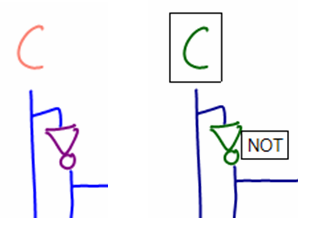
\includegraphics[width=.65\linewidth]{feedbackDemo.png}
  \caption{\label{fig:feedbackDemo}
           Text and color feedback comparison.}
\end{figure}

%\subsection{Specifying Strokes to Recognize}

The second issue we explored was how to allow the user to indicate
which strokes the system should recognize.  It is possible to provide
separate sketching panels for notes and diagrams, but when users want
to make annotations directly on the diagram, this setup is infeasible.
We examined two techniques for allowing users to segregate
recognizable strokes from unrecognized strokes:

\begin{itemize}
\item \textbf{Pre-separation: ``Color'' Tool.} This version of the
  interface requires users to separate domain strokes from
  annotation strokes as they draw by toggling between stylus
  modes using a button on the GUI.  The system uses ink color to indicate the
  current mode: in sketch mode, the stylus draws black ink; in
  annotation mode, the stylus draws gray ink (hence we call this
  option the ``color'' tool).
\item \textbf{Post-separation: Lasso Tool.} The user draws sketches
  and annotations freely, but then must lasso-select strokes to be
  recognized (similar to the interaction mechanism in
  MathPad$^{2}$\cite{LaViola2006Initial}).  
\end{itemize}

%\subsection{Feedback Mechanisms}
The third issue we explored is how to display recognition feedback.
We compared two different methods: color feedback and text labels
(Figure~\ref{fig:feedbackDemo}).  We rejected the idea of replacing
the user's strokes with symbols based on lack of common interest in
this idea during pre-studies and the results of previous
work~\cite{Hong2002Sketch}.

\begin{itemize}
\item \textbf{Color Feedback.} The system displays each recognized
symbol in a unique color.  In addition, users can see a text label by
hovering the stylus over the strokes in the symbol.  
\item \textbf{Text-Label Feedback.}  The system draws text labels next
to recognized symbols.
\end{itemize}


%% \textit{I took out these sentences because I'm not sure we want to
%%   hypothesize here.}
%% Color: We conjecture that this
%% feedback mechanism might prove the easiest to interpret and the most
%% comfortable to visually recognize.  

%% Text: We conjecture that this
%% feedback mechanism might prove the easiest to interpret and the most
%% comfortable to visually recognize.  

%\subsection{Impact of Recognition Error}
Finally, we investigated how three types of common recognition errors
impact the user experience: false positives, false negatives and
stroke grouping errors (Figure \ref{fig:errorDemo}).  False positives
occur when the system incorrectly identifies a symbol (e.g., labels an
AND gate as an OR gate); false negatives (or \textit{omissions}) occur
when the system fails to identify a symbol; and grouping errors occur
when the system incorrectly adds or removes adjacent strokes to or
from a symbol.


\begin{figure}[tb]
  \centering
  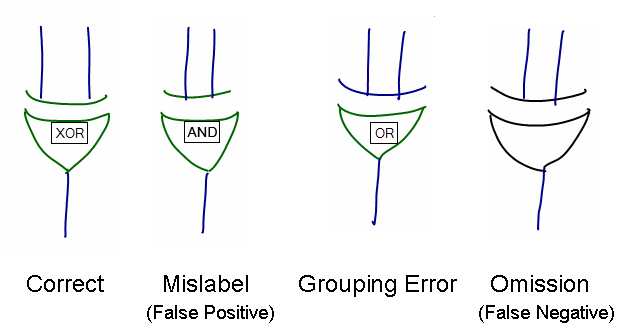
\includegraphics{errorDemo.png}
  \caption{\label{fig:errorDemo}
           Illustration of different error types.}
\end{figure}

%-------------------------------------------------------------------------
\section{Experimental Design}
For this study, we limited our scope to digital circuit design in order
to keep tasks consistent across all users so as to better
understand how interface decisions (as opposed to domain variability)
affect usability.  Although focusing on a single domain limits the
generality of our results somewhat, the style of the tasks we
explored is representative of structured educational design tasks 
in many fields, such as the sciences and engineering.

\subsection{Tasks and Participants}
Users in our study designed circuits based on truth table function
representations---a common task in an introductory digital design
class.  Figure~\ref{fig:tt-task} gives an example of one of these
tasks.  Users were allowed to use any method to
create the circuit, and they were not required to simplify their
circuit (although they could if they wanted to).  In some cases
(described in Section~\ref{sec:design}) we also asked uses to annotate the
shortest and longest path through the circuit they designed.



 \begin{figure}[tb]
 \centering
 \begin{tabular}{p{.85\linewidth}}
 	Please draw a circuit diagram for the following truth table:
 	\end{tabular}

   \subfigure[Truth table task] {
   	\label{fig:tt-task}

 			
      \begin{tabular}{|l|l|l||l|l|}
      \hline 
      \multicolumn{3}{|c||}{Input} & \multicolumn{2}{c|}{Output} \\
      \hline
      A & B & C & F & G \\
      \hline
      0 & 0 & 0 & 0 & 1 \\
      \hline
      0 & 0 & 1 & 0 & 0 \\
      \hline
      0 & 1 & 0 & 0 & 1 \\
      \hline
      0 & 1 & 1 & 0 & 0 \\
      \hline
      1 & 0 & 0 & 0 & 0 \\
      \hline
      1 & 0 & 1 & 0 & 0 \\
      \hline
      1 & 1 & 0 & 1 & 0 \\
      \hline  
      1 & 1 & 1 & 1 & 1 \\
      \hline        
    \end{tabular}
} 
   \subfigure[A possible solution (with color feedback).  The black dot
     denotes the user's stylus.] {
     	\label{fig:tt-solution}
 	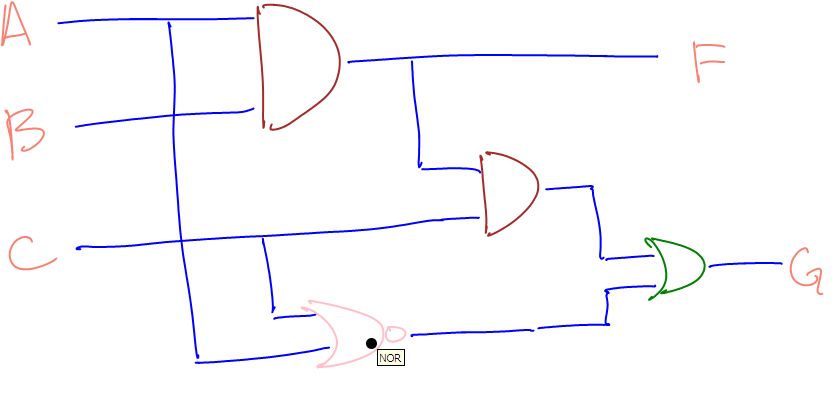
\includegraphics[width=0.8\linewidth]{complete.png}  
   }
 	\caption{ A truth table task from our user study}
	\label{fig:task}
 \end{figure}


%\begin{figure*}[tb]
%  \centering
%  \subfigure[Truth table task]{
%  	\label{fig:tt-task}
%    \textit{Given the truth table below, sketch the corresponding schematic}
%    \begin{tabular}[|l|l|l|l]
%      \hline 
%      \multicolumn{3}{l}{Input} & Output \\
%      \hline
%     0 & 0 & 0 & 0 \\
%     \hline
%     0 & 0 & 1 & 1 \\
%     \hline
%      0 & 1 & 0 & 0 \\
%      \hline
%      0 & 1 & 1 & 0 \\
%      \hline
%     1 & 0 & 0 & 1 \\
%      \hline      
%    \end{tabular}
%    \label{fig:tt-task}
%  }
%  \subfigure[Possible solution]{
%%    \includegraphics[width=0.5\linewidth]{Figures/instr_060130_slide11}
%    %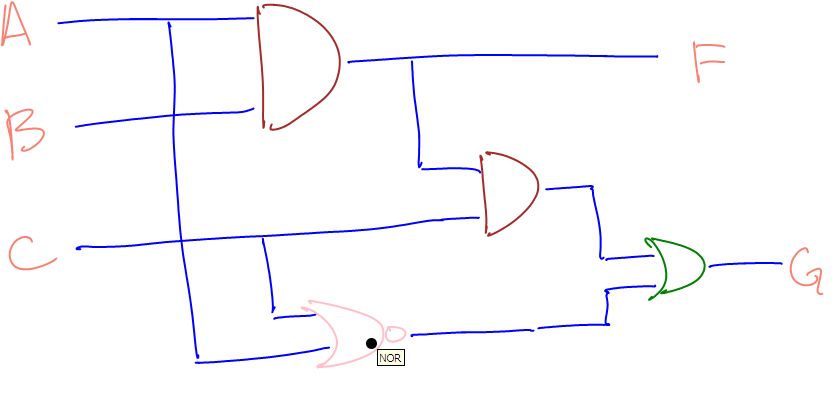
\includegraphics[width=\linewidth]{complete.png}
%    \label{fig:tt-result}
%  }
%  \caption{A task from our user study}
%  \label{fig:task}
%\end{figure*}


We used a pre-study to design a set of uniformly difficult tasks.  We
asked participants to rate the difficulty of several tasks and
selected for our study only those tasks that users rated as similarly
difficult.  Participants reported that these tasks were similar in
difficulty to typical homework problems in an introductory digital
design course.

%% Users completed a fixed set of circuit design tasks.  For each task we
%% varied one aspect of the user interface.  We describe the details of
%% each of the user interface elements we varied below.  Each participant
%% completed between three and five tasks, and each session lasted 45-60
%% minutes.

In total, nine people (six male and three female) participated in our
formal tests (not including the pre-studies). All participants were
Harvey Mudd College students who had taken an introductory digital
circuit design class.  All participants had used digital circuit
simulation software (Xilinx) in their coursework.  Six of these
students had previous experience (more than an hour) with a Tablet PC,
and five had taken notes on a Tablet PC during their digital design
course (using Windows Journal or One Note).

\subsection{Basic Interface Design}
We first designed our prototype interface using iterative design
techniques.  Figure~\ref{fig:fullGUIdemo} shows a basic overview of
our final interface, although we modified pieces of this interface to
explore different interface elements.  In this version, the user
sketches (unrecognized) notes in the bottom panel, sketches the
(recognized) circuit in the top panel and presses the ``Recognize''
button to trigger recognition.


\begin{figure}[tb]
  \centering 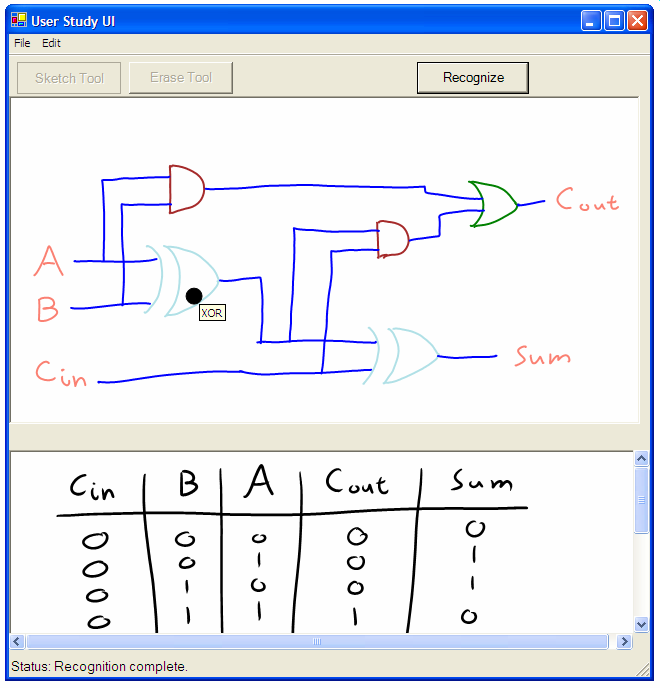
\includegraphics[width=0.85\linewidth]{fullGUIdemo.png}
  \caption{Complete sketch recognition interface. }
  \label{fig:fullGUIdemo}
\end{figure}


Users could correct recognition errors only by erasing and redrawing
their strokes.  We did not aim to explore error correction mechanisms,
and this method was adequate for users to complete their tasks.
However, error correction mechanisms deserve attention from future studies as
they are an important element of sketch recognition interfaces.


%% Not needed--too much detail.  In general, only talk about what
%% you actually did, not what you planned to do.

%% Furthermore, the manual correction of errors can itself be a
%% frustrating process.  Participants of our paper prototype study
%% suggested several different correction mechanisms.  Potentially useful
%% correction mechanisms include:\\

%% \textbf{Correction Mechanisms} 
%% \begin{itemize}
%% \item \textbf{Gesture Correction} Users use a gesture to erase a
%% symbol.  For example, a user could cross out a symbol with an 'X' or
%% lasso the symbol and draw a straight line through the lasso to
%% indicate deletion.
%% \item \textbf{Multi-Modal Correction} Users could press a button to
%% toggle the stylus from drawing mode to eraser mode
%% \item \textbf{WIMP-Based Correction} Users press a button while
%% tapping on a symbol in order to trigger a menu of alternate labels for
%% the symbol.
%% \end{itemize}

%% A thorough examination of these correction mechanisms would likely
%% require an extended study of prolonged use in order to gain insight
%% into the efficiency of these mechanisms.  For the purposes of our
%% study, we required users to correct errors using an erase-and-redraw
%% process that entailed using the erase feature of the stylus.


\subsection{User Studies}
\label{sec:design}
We conducted two separate studies to investigate the four interface
elements described above. In the first study we investigated
recognition triggers and diagram separation tools.  In the second
study we examined recognition feedback and error types. We divided our
investigation into two studies in order to minimize the mental burden and
scheduling commitment on users.

During both user studies we invited all participants to contribute
informal feedback and asked them to fill out questionnaires inspired
by the previous work of Chin et al.\cite{chin88} and
Landay\cite{landay96thesis}.  Our questionnaires aim to measure user
responses to individual interface elements based on relevant
characteristics we inferred from our pre-study interviews and related
work in sketch recognition user interfaces.

\subsubsection{User Study \#1: Recognition Triggers and Diagram
  Separation} 

Our first study examined triggers and diagram separation preferences
across five participants.  Each participant completed one truth table
task with each recognition trigger using the multi-paneled interface
depicted in Figure \ref{fig:fullGUIdemo}; the order of triggers tested
was balanced across participants.  Next, each participant completed
one truth table task with each diagram separation tool in a
single-paneled version of our interface.  We prompted participants to
label the shortest and longest path in their circuits and to have the
system recognize only their diagrams (e.g., not the annotations).

After each task, the experimenter prompted users for qualitative
feedback and gave questionnaires asking users to rank the reliability,
efficiency, convenience and overall quality of the interface.  After
completing all tasks, users ranked their preferred feedback and
diagram separation mechanisms.  Users completed study sessions in
30-45 minutes.

This study used two methods to ``recognize'' the user's diagrams and
gestures.  First, our system recognized users' check-tap gestures
using the built-in Microsoft Tablet SDK gesture recognizer.  Some
users' gestures were recognized reliably, but others were not (we
discuss the implications below).  Second, the system simulated
recognition of the users' diagrams by coloring most of the strokes
blue, indicating ``correct recognition,'' but displaying approximately
10\% of the strokes in red, indicating a ``recognition error.''  No
recognition actually occurred, but most users expressed that they genuinely presumed
the recognition results and simulated errors were real.

\subsubsection{User Study \#2: Feedback Mechanisms and Error Types}
Our second study examined recognition feedback and recognition errors
across six participants (including two participants from our first
study).  Each participant again completed one truth table task per
feedback method and per error type, and we balanced the order of
feedback mechanisms and error types, respectively, across users.
(Feedback tasks always preceded error tasks.)  When completing the
error tasks, users chose the feedback mechanism they preferred.  In all
tasks, users triggered recognition with a button. 

Again after each task, the experimenter prompted users for qualitative
feedback and gave them questionnaires asking them to assess the
reliability, efficiency, convenience and overall quality of the
interface.  After completing all tasks, users ranked which feedback
mechanism they preferred and which errors were most confusing or
difficult.  Users completed study sessions in 45-75 minutes.

This study simulated diagram recognition through a novel application
of a Wizard of Oz technique.  Users worked with a realistic Tablet PC
application while a human ``Wizard'' actively labeled user-drawn
symbols.  Wizard of Oz studies have proven effective for
developing speech recognition interfaces~\cite{169968,354406}, but
this is the first application of Wizard of Oz studies to the design of
sketch recognition systems of which we are aware.  Davis has developed a 
Wizard of Oz system to support sketch recognition user interface 
development\cite{Davis2007SketchWizard},
but this system was not ready in time for our study.  

Our experimental Wizard of Oz system consists of two Tablet PCs directly 
networked over an Ethernet connection.  As the user sketches on one Tablet, the
Wizard actively receives copies of user strokes and labels relevant
symbols on a second tablet.  Once the user triggers recognition, the
Wizard sends a labeled result to the user Tablet.  For this stage of
our study, our human subjects committee required us to inform
participants that a human was recognizing their strokes.

%% Our prototype user interface and wizard labeling system were both
%% developed in in C\# 1.1, using Microsoft\textregistered \ Visual
%% Studio\textregistered \ .NET 2003.  Both user and Wizard used HP
%% Compaq tc4200 Tablet PCs running Microsoft\textregistered \
%% Windows\textregistered \ XP Tablet PC Edition 2005.

The Wizard simulated perfect recognition while participants tested
feedback mechanisms.  To test error types, we simulated a 15\%
(approximate) error rate.  We chose this rate because it is a
realistic target for sketch recognition systems in the near future.  We
simulated each error type as follows:
\begin{itemize}
\item \textbf{False Positives.} The user end of our Wizard
of Oz system filtered recognition results from the Wizard and randomly
applied incorrect labels to approximately 15\% of the
recognition result.
\item \textbf{False Negatives.} The system again filtered the Wizard's simulated results,
randomly deleting the labels from approximately 15\% of symbols.
\item \textbf{Grouping Errors.}  The
Wizard incorrectly grouped the strokes in
approximately 15\% of symbols drawn, usually giving about 3 to 4
grouping errors per sketch.  
\end{itemize}


%-------------------------------------------------------------------------
\section{Results and Discussion}
In this section we present select quantitative and qualitative results
of our study.  Space constraints prohibit us from including complete
user response data.  In part due to our small sample size, even when users
agreed, many of our survey responses do not show statistically
significant differences.  In many of these cases, however, qualitative
feedback supports patterns in quantitative results.  When users had 
conflicting opinions, we summarize these different beliefs so as to inform
interface designers about the range of user preferences.

\subsection{Student Workflow}

Students unanimously reported that they prefer to design their
circuits on a Tablet PC or whiteboard rather than enter them directly
into a simulation tool.  Furthermore, during our study, all of our
participants used almost identical workflows.  When designing a
circuit, each student would write notes or equations, sketch a
circuit, trigger recognition, and then correct recognition errors.
Even when the experimenter reminded users that they could trigger
recognition intermittently during the design process, participants
continued to trigger recognition only after sketching a complete or
significant portion of a circuit.  User comments reveal two reasons
for this workflow: users prefer to focus on the design and
sketching portions of their tasks without interruption, and they
prefer to correct recognition errors in a batch instead of
individually.  

% Not sure if this text has a home.  The comment on Pause trigger
% should go with that discussion.  
%  Another
%user found the Pause Trigger excessively irritating and commented that
%"[recognition] happened when [she] was doing other
%things---distracting."  Another user compared using the tool to
%iteratively writing and compiling software code with an IDE.  This
%user commented that he only triggered recognition after verifying his
%completed sketch because he "fe[lt] like [he] should give it something
%that runs."  


\subsection{Recognition Triggers}

%% \begin{table}
%%   \centering
%% 	\begin{tabular}{|p{.35\linewidth}|c||c||c|}
%% 	\hline 
%%   Question 																									& Button & Gesture & Pause \\
%%   \hline
%%   This trigger was convenient to use. 											& $5.3\pm0.4$ & $4.1\pm2.2$ & $5.4\pm0.9$ \\
%%   \hline
%%   I felt comfortable using this trigger. 										& $6.4\pm0.9$ & $5.9\pm1.4$ & $5.4\pm1.8$ \\
%%   \hline
%%   This trigger was reliable.																& $7.0\pm0.0$ & $3.2\pm2.5$ & $5.6\pm1.5$ \\
%%   \hline
%%   This trigger was efficient.																& $5.6\pm0.5$ & $4.4\pm2.4$ & $5.0\pm1.2$ \\
%%   \hline
%%   My experience using this trigger was satisfying.					& $6.1\pm0.5$ & $5.0\pm2.0$ & $4.4\pm1.5$ \\
%%   \hline
%% 	\end{tabular}
%% 	\caption{Questionnaire results for recognition triggers.  Users are asked to express their feeling on a scale of 
%% 	1 = strongly disagree to 7 = strongly agree.  Standard deviations are given in survey points.}
%% 	\label{tab:TableATriggerData}
%% \end{table}


% We conjecture that users might find gesture-based triggers more convenient, efficient, and natural. 
%% Table~\ref{tab:TableATriggerData} summarizes users' responses to
%% different recognition triggers.  

User reactions suggest that high reliability is the most important
characteristic of a recognition trigger.  Most users were able to 
successfully trigger recognition using check-tap only once
for every five failures. Though users admit the gesture trigger offers
a desirable convenience, the majority of users
(n=3) ranked the button trigger higher than the other two triggers,
and users unanimously rated it as highly reliable (Figure
\ref{fig:buttonReliabilityChart}).

The button trigger's high reliability minimizes users' mental effort
and allows them to devise efficient workflows.  One user commented
that the button trigger helped her make her ``approach more
systematic'' and ``figure[] out [the] most efficient way to'' use the
interface.  A second user commented that ``[he could] always get
faster with a tool that works every time.''

The relatively high error rate of the check-tap gesture colored many
users' reactions to this trigger.  The one user that ranked the
gesture trigger as the most desirable was able to trigger recognition
successfully on his first six attempts.  Even still, this user
admitted to seeing only a ``marginal difference'' between the gesture
and button triggers.

User reactions to the pause trigger suggest that students may
find the pause trigger acceptable only if it matches the speed of their
thought processes.  Two users commented that a four second pause was
too long, while one user found the pause trigger quite ``distracting''
to her mental flow and suggested a longer pause.  The one user who
ranked the pause trigger as his favorite trigger commented that it
allowed him to ``check as [he] move[d] through creating the diagram.''

\begin{figure}[tb]
  \centering
  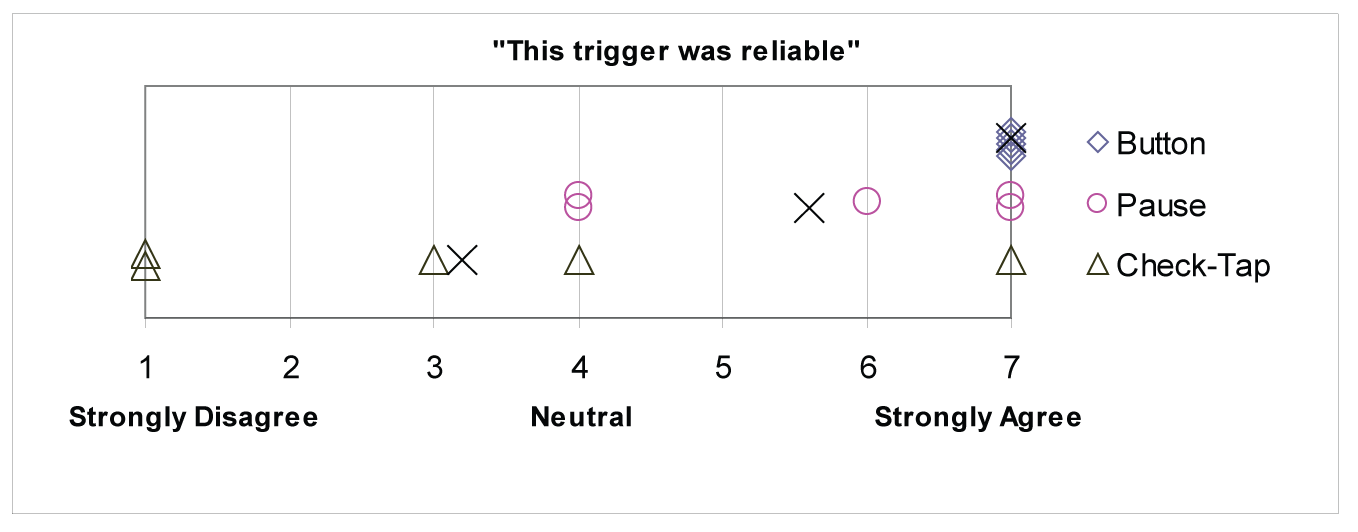
\includegraphics[width=1.0\linewidth]{buttonReliable-bigger.png}
  \caption{\label{fig:buttonReliabilityChart} Individual user responses
           to recognition trigger reliability. Each symbol represents
           a single user's response.  ``X''s show mean values.}
\end{figure}

%% Quotes not used:
%% Another user commented with frustration that the Gesture
%%Trigger was "very unreliable" and that the Button Trigger was
%%(desirably) much more "consistent."  

 \subsection{Separation/Annotation Tools}

%% \begin{table}
%%   \centering
%% 	\begin{tabular}{|p{.45\linewidth}|c||c|}
%% 	\hline 
%%   Question 																									& color tool & Lasso Tool \\
%%   \hline
%%   This annotation tool was convenient to use.								& $6.2\pm0.4$ & $3.2\pm1.3$  \\
%%   \hline
%%   I felt comfortable using this annotation tool.						& $6.6\pm0.5$ & $5.0\pm1.0$  \\
%%   \hline
%%   This annotation tool was reliable.												& $6.0\pm1.0$ & $4.0\pm1.4$  \\
%%   \hline
%%   This annotation tool was efficient.												& $6.5\pm0.5$ & $3.4\pm1.1$  \\
%%   \hline
%%   My experience using this annotation tool was satisfying.	& $6.2\pm0.8$ & $3.4\pm1.1$  \\
%%   \hline
%% 	\end{tabular}
%% 	\caption{Questionnaire results for Annotation Tools.}
%% 	\label{tab:TableBAnnotationData}
%% \end{table}


%% Table~\ref{tab:TableBAnnotationData} summarizes user response to
%% survey questions about separation techniques.  
Users unanimously preferred the pre-separation (color) tool to the
post-separation (lasso) tool, and all users found the pre-separation
tool more satisfying to use than the post-separation tool (Figure
\ref{fig:annotationSatisfaction}).  Many modal interfaces
traditionally suffer from the problem that users often forget to
toggle to the appropriate mode before performing a task.  However, in
our study, only one of five users forgot to toggle the color tool into
annotation mode before writing notes; furthermore, this user corrected
her mistake immediately.

Two participants commented that the lasso tool constrained the way
they could create their diagrams.  One user described that
the color tool "required less planning about where and when to write
so as not to screw up [the] lasso[] [gesture]."  Another user
commented that she ``like[d] the [color tool's] ability to draw
annotations wherever [she wanted].''

One issue that may have influenced user responses to the separation
mechanism is that the lasso tool required two check-tap gestures while
the color tool required only one.  Nevertheless, users responded more
negatively to the burden of circling the symbols and the physical
segregating of annotation and schematic strokes than to executing the
gesture.  One user even modified her questionnaire to express her
preferences for annotation tools that hypothetically used the button
trigger rather than check-tap; this user still preferred the color
tool.

%I don't think you need this part.  
% Two users noted that
%both annotation tools suffered from the lack of reliability of the
%Check-Tap Gesture.  Operation of the Lasso Tool requires execution of
%two Check-Tap gestures while operation of the color tool requires only
%one.  Though the reliability issue surrounding the Check-Tap gesture
%colors user reactions to the annotation tools, the fact remains that
%the Lasso Tool requires more effort in circling symbols and the
%physical segregating of notes and schematic strokes.  Clearly the
%potential for confusion over the multi-modal nature of our
%Pre-separation tool imposed a minimal and acceptable burden on users.

\begin{figure}[tb]
  \centering
  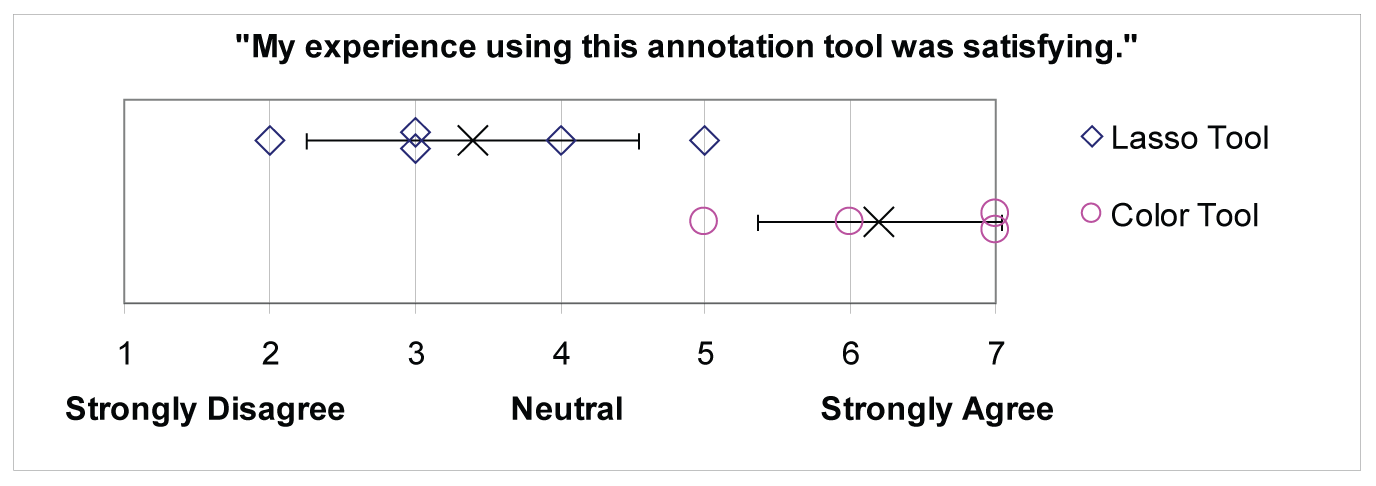
\includegraphics[width=1.0\linewidth]{annotationSatisfying.png}
  \caption{\label{fig:annotationSatisfaction} Individual user
           responses to sketch separation method satisfaction.  Error bars are shown for
           one standard deviation.}
           
\end{figure}



\subsection{Feedback Mechanisms}

%% \begin{table}
%%   \centering
%% 	\begin{tabular}{|p{.45\linewidth}|c||c|}
%% 	\hline 
%%   Question 																									& Color & Text-Label \\
%%   \hline
%%   This feedback mechanism produced understandable results.	& $7.0\pm0.0$ & $6.5\pm0.5$  \\
%%   \hline
%%   I would feel comfortable submitting the result on my screen as a diagram for my homework.
%%   																													& $6.5\pm0.5$ & $5.0\pm1.9$  \\
%%   \hline
%%   This feedback helps me work efficiently.									& $6.3\pm1.2$ & $5.1\pm1.6$  \\
%%   \hline
%%   The feedback was distracting.															& $1.1\pm0.4$ & $3.1\pm2.4$  \\
%%   \hline
%%   The feedback was confusing.																& $1.3\pm0.5$ & $2.1\pm1.6$  \\
%%   \hline
%%   My experience using with this feedback mechanism was satisfying.
%%   																													& $6.5\pm0.5$ & $5.5\pm1.9$  \\
%%   \hline
%% 	\end{tabular}
%% 	\caption{Questionnaire results for Feedback Mechanisms.}
%% 	\label{tab:TableC1FeedbackData}
%% \end{table}


%% Table~\ref{tab:TableC1FeedbackData} summarizes user survey responses
%% to feedback mechanisms.  

Users unanimously agreed or strongly agreed that color feedback
``helped them work efficiently'' and ``produced understandable
results''; most users preferred color feedback to text-label
feedback.  Users found text feedback distracting (Figure
\ref{fig:feedbackDistracting}) and that it added an unnecessary
mental burden to the design process.  One user commented that ``The
text gets very cluttered [and] covers up the [sketch's] points of
interest quickly,'' thus interrupting his ability to reason about the
diagram.  Another user commented that text labels ``can get a little
distracting with four or five [instances] of the same gate'' and finds
the color feedback ``more elegant'' and ``less redundant.''  Although our
specific text placement may have influenced user perception of the
text labeling feedback mechanism (i.e., sometimes the text obscured
part of the sketch), automatic text placement is a difficult problem,
and any automatic text placement method will likely obscure some
portion of the user's sketch.

%% Furthermore, the cluttering issue surrounding Text Feedback suggests
%% users might have expressed equal disdain for feedback through stroke
%% substitution (e.g., through Symbol Replacement).  We did not develop
%% and test Symbol Replacement due to the lack of common interest in this
%% feedback during our paper prototype study; furthermore, Symbol
%% Replacement Feedback presented technical challenges that would make
%% development impractical for our project's timeframe.  Originally we
%% had considered two possible implementations for Symbol Replacement:
%% one implementation that faintly overlays symbols over a sketch and one
%% implementation that completely erases and replaces user strokes with
%% symbols.  The overlay implementation would have entailed even more
%% sketch obfuscation than that of text labels, thus we anticipate that
%% users would still have preferred Color Feedback.  Moreover, the
%% obfuscation issue that our users raise negates an implementation that
%% entails complete stroke replacement.  Complete stroke replacement
%% would necessarily destroy user strokes and completely prevent users
%% from comparing recognition result labels (e.g., B\'{e}zier Curve
%% symbols) to raw ink symbols.

Despite the distracting nature of text feedback, color feedback alone
is likely not informative enough.  During the color feedback tests,
each of the six participants immediately hovered her or his stylus
over individual gates to verify the labels.  In
addition, one user commented that she ``like[d] both'' methods of
feedback and found that ``a button to go back and forth [between
feedback mechanisms] would be nice.''

%% The
%% informal responses of three other participants corroborate the
%% usefulness of a feature for toggling text labels.  On the other hand,
%% one user specifically opined against such a toggle feature because he
%% found the obfuscation of text feedback made this type of feedback
%% impractical for use.  However, the (sole) user who ranked text
%% feedback as the most desirable asserted that the text labels did not
%% bother him and that "It's easier to distinguish gates by their name
%% rather than [through the use of] different colors."

%% However, color feedback alone is not enough.  

\begin{figure}[tb]
  \centering
  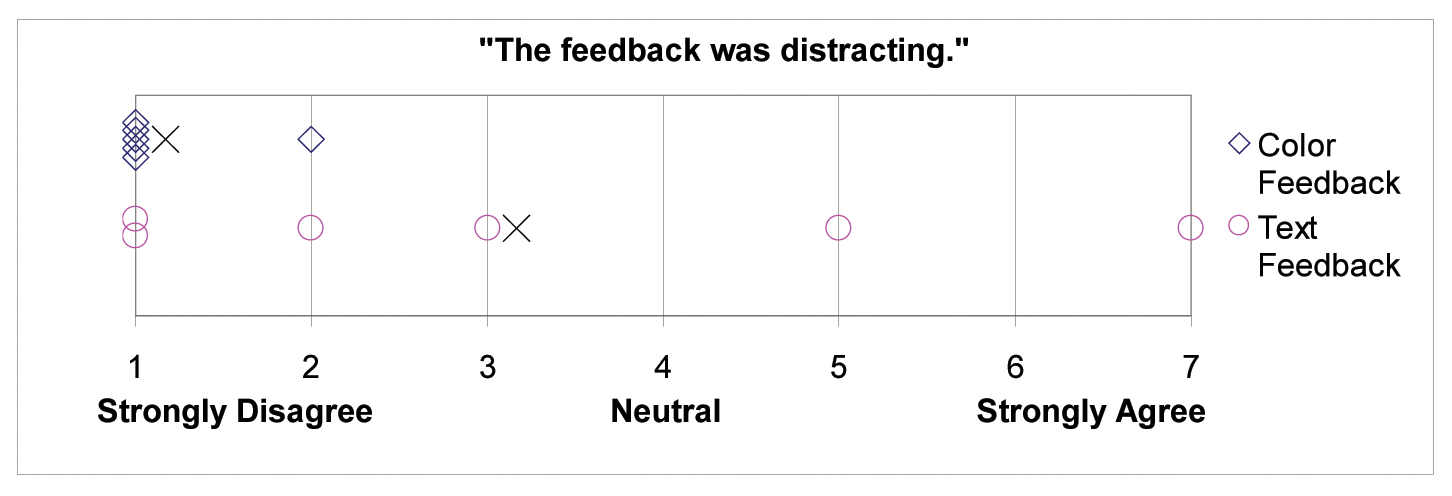
\includegraphics[width=1.0\linewidth]{feedbackDistracting.png}
  \caption{\label{fig:feedbackDistracting}
           Individual user responses to feedback distraction.}
\end{figure}

%% Unused text:
%In contrast, this user found the "hover"
%feature of Color Feedback "less distracting."  The text labels'
%obfuscation of the sketch causes user distress.  In response to the
%issue of obfuscation, one user exclaimed that he "[couldn't] tell what
%gate [he] drew [when he drew] small gates."  Obfuscation taints the
%Text Feedback's aesthetic.  

\subsection{Error Types}


%% \begin{table}
%%   \centering
%% 	\begin{tabular}{|p{.35\linewidth}|c||c||c|}
%% 	\hline 
%%   Question 																									& Mislabel & Omission & Group \\
%%   \hline
%%   Detecting errors was difficult. 													& $2.3\pm1.0$ & $2.6\pm1.9$ & $3.5\pm1.2$ \\
%%   \hline
%%   These errors frustrated me. 															& $4.5\pm2.2$ & $4.0\pm2.0$ & $4.1\pm1.3$ \\
%%   \hline
%%   Correcting errors was cumbersome. 												& $3.8\pm1.6$ & $2.8\pm1.5$ & $3.0\pm1.9$ \\
%%   \hline
%%   I attempted to understand why the system produced errors.	& $3.0\pm1.9$ & $3.3\pm1.6$ & $3.3\pm2.7$ \\
%%   \hline
%%   If I continued to encounter this type of error during further use of this application, I would change how I sketch.																																					& $3.0\pm2.1$ & $3.6\pm1.8$ & $4.8\pm1.7$ \\
%%   \hline
%%   These recognition errors confused me.											& $3.5\pm2.1$ & $3.0\pm1.9$ & $3.0\pm1.3$ \\
%%   \hline
%% 	\end{tabular}
%% 	\caption{Questionnaire results for error types.}
%% 	\label{tab:TableDErrorData}
%% \end{table}




%Figure \ref{fig:errorChangeSketch} indicates that users tended to be
%more willing to adapt their sketching styles in response to grouping
%errors.  Though three of six users expressed that they would be
%willing to adapt to the system in order to reduce errors, qualitative
%user reactions were not as consistent.

Users had diverse reactions to recognition errors, and our
quantitative results show no strong trends.  This lack of quantitative
trends may be due in part to an unintended effect of the way we
generated errors.  To keep error rates consistent, the computer system
automatically generated omissions and false positives.  However,
generating grouping errors was too difficult to automate (it would
require a deeper understanding of the sketch in order to split and
merge adjacent groups), so the human Wizard generated grouping errors.
Consequently, false positives and omissions were often more surprising
to users (e.g. a wire classified as an AND gate) than grouping errors.
This effect limits the direct comparison we can make between user
responses to error type, but allows us to better understand the
importance of how users perceive errors based on how well they
understand them.

Our qualitative results suggest that user acceptance of the system is
related not only to absolute error rates but also to how well they
understand and trust the system's recognition.  Generally, our users
were initially happy to correct any type of recognition error, but
quickly became frustrated when they could not understand why errors
occurred.  Two users specifically explained that their acceptance of
the system would depend not on the error rate as much as on the
predictability of errors.  One of these users remarked that he would not be
willing to accept a system with the error rate exhibited unless errors
were more predictable and helped him adapt his drawing style to avoid
them.  This user also found false negatives the most confusing because
these errors failed to inform him about ``what to move away from''
(i.e., how to change his sketching style to reduce errors).  On the
other hand, another user preferred false negatives because it made him
trust the system more when it did recognize his strokes.  Though related 
work suggests that user acceptance may improve with lower absolute error
rates, our results illustrate the importance of user perception of 
error type to acceptance of the system.  Future work may seek to further 
compare the impacts of error type and error rate on user experience.  

%END: contemplating related work... would improved error rate really have
%minimized the frustration of crazy 'xor' wires... e.g. would error rate 
%really have an impact here?  hmmm

%% User frustration with errors stems from the inability to establish a
%% reliable and practical mental model of errors.  Generally, users are
%% initially happy to correct any type of recognition error.  Repeated,
%% frustrating errors will inspire users to commit modest yet pragmatic
%% mental effort to understanding errors.  If users fail to learn to
%% predict errors, then frustration will lead them to distrust and reject
%% the system.  Indeed, we found that acceptance of this tool hinged on
%% frustration with, and the predictability of, errors.  Two users
%% remarked that they would accept the current error rate as-is.  Another
%% user also expressed acceptance of the current error rate and remarked
%% that the time required to correct recognition errors with our system
%% was comparable to the time she spent correcting errors while using the
%% WIMP applications her coursework requires.  One user specifically
%% rejected our interface based upon the exhibited error rate and
%% specified that he would only find one recognition error per circuit
%% schematic acceptable; however, this user responded that he was only
%% "kind of" able to predict errors.  The remaining two users both
%% explained that their acceptance of the system depended heavily on the
%% predictability of errors.  One user explained that he would accept the
%% system only if he could reasonably "adapt to" it and that he wanted
%% system errors to help inform his drawing style.  The other emphasized
%% the impact that error rate had on his trust of the system.  This user
%% explicated that he would trade a higher omission error rate for lower
%% grouping and mislabel error rates.  He explained that "if [the system]
%% says 'I don't know what [a sketched symbol] is' then that's a good
%% thing"; a tendency to omit labels rather than incorrectly assign
%% labels helps make the system "safer" to use.  The predictably and
%% acceptance of errors is crucial to an interface's trustworthiness.



We also found that users created dramatically different mental models
of errors.  Two users considered themselves responsible for grouping
errors.  Two users blamed the system for mislabel and omission errors.
One of these users remarked that mislabel and omission errors seemed
``out of context,'' or unpredictable.  Two users specifically remarked
that they did not try to form a mental model of errors.

Qualitative user responses related to frustration with errors
exhibited a general accordance.  Four out of six users responded that
omission errors were the easiest to perceive; users likely find that
the lack of a label is easier to detect than an incorrect label.
Furthermore, four out of six users remarked that the grouping error
was the most confusing type of error despite the fact that these
errors were human-generated.


%% Three users indicated that they would be
%% inclined to change their sketching styles in order to deal with
%% grouping errors (see Figure \ref{fig:errorChangeSketch}).  One user
%% who responded positively to this survey question (giving a rating of
%% 7/7) also found grouping errors the most confusing; however, this user
%% explained her reaction as a result of the fact that grouping errors
%% were her first exposure to errors.  Two other users who responded
%% positively to the survey question (both giving a rating of 6/7)
%% remarked that they did not attempt to form a mental model of errors.
%% Therefore, users who found grouping errors the most confusing gave
%% survey responses that they were the least likely to change their
%% sketching styles in reaction to grouping errors. \textit{This needs
%% more explanation--it's a little confusing}

%% % plot for survey question "I would change my sketching style of these errors continued..."
%% \begin{figure}[tb]
%%   \centering
%%   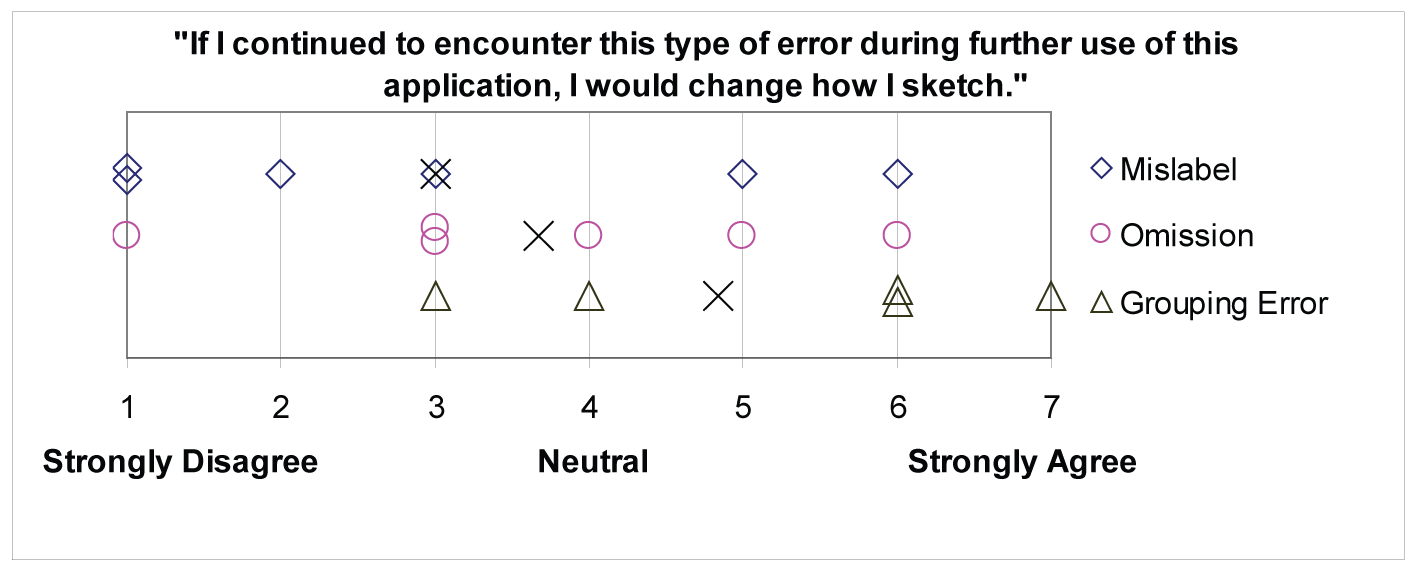
\includegraphics[width=1.0\linewidth]{errorChangeSketch.png}
%%   \caption{\label{fig:errorChangeSketch}
%%            Individual user responses to whether or not they
%%            would change their sketching style}
%% \end{figure}

%User reactions to other types of errors corroborate a trend that
%confusion leads to rejection of the system.  Expressing angst over the
%unpredictability of the randomly generated mislabel errors, one user
%asserted that "[he] would probably not change [his drawing] techniques
%to match the tool, [he'd] just not use the tool."  This user also
%specifically explained that his acceptance of the system would depend
%on the predictability of errors.  Another user expressed similar angst
%with mislabel errors and commented that they were   ; this user was willing to adapt his style to the
%system but explains that the lack of a correct or incorrect label
%fails to enable him to change his style.  

%% Finally, the error correction process also impacted user reactions to
%% the system.  Three users remarked that more effective error correction
%% mechanisms would help ameliorate the frustration of dealing with
%% errors.  Though most users were comfortable using the erase gesture to
%% erase and redraw incorrectly recognized symbols, one user found the
%% erase gesture hard to control because of the size of the stylus'
%% eraser.  Another user requested a selection tool for erasing large
%% amounts of ink.

%%  and the final user requested support for debugging
%% circuit connections.  The remaining user specifically requested a 'netlist'
%% feature that would allow a user to visually highlight and debug
%% connections between symbols.  This 'netlist' feature would both aid in
%% the verification of a circuit design and help users detect grouping
%% errors.
  



%-------------------------------------------------------------------------
%% \section{Error Analysis}
%% \textit{This stuff should be integrated into the text above, rather
%%   than presented as one big disclaimer at the end.  I've tried to do
%%   this and commented out the stuff that I think is integrated (see
%%   comments in the latex source).  Are
%%   any of our results statistically significant?}

% I think I covered most of this paragraph in the first part of the
% results section. 
%% Most of our survey data fails to provide a statistically significant
%% foundation for the identification of solid trends in user preferences.
%% Furthermore, in some cases our users presented conflicting viewpoints
%% in response to qualitative questions.  Most traditional evaulation
%% techniques and questionaires measure the overall performance of an
%% application with respect to well-established axes of macroscopic
%% system characteristics (I have no reference for this, its just an
%% observation).  However, our study breaks new ground in attempting to
%% inform system design through the juxtaposition of contrasting
%% interface elements.  Through our evaluation measures and experimental
%% methodology, we have more effectively illuminated apposite axes of
%% interface element characteristics than measured against an existing
%% metric.

% This paragraph is covered with the presentation of results.
%% The unreliability of the Check-Tap gesture confounded user reactions
%% to Recognition Triggers and Annotation Tools.  This confounding
%% prevents conclusively determining one Recognition Trigger or one
%% Annotation Tool as maximally efficacious.  However, our inquiry
%% illuminates how the efficacy of Recognition Triggers and Annotation
%% Tools are directly related to how well these interface elements
%% support efficient work.  Despite the exceptionally high gesture error
%% rate observed, the emphasis of user responses on the importance of
%% reliability suggest that gestures may make inherently impractical
%% Recognition Triggers.  Furthermore, qualitative user feedback
%% comparing the Color and Lasso Annotation Tools emphasizes users'
%% preference for efficiency and simplicity.  Users see convience and
%% novelty as secondary characteristics.

% Incorporated above.
%The implementation of the Text-Label Feedback partially counfounded
%legibility of recognition results.  Two users complained that text
%labels often made recognition results illegible because labels would
%completley obfuscate small gates.  Despite this quirk, any labeling
%method will entail some amount of obfuscation of the sketch.  User
%responses emphasize the importance of the minimization of distracting
%aspects of feedback, therefore any label-based Feedback Mechanism may
%fail to maximize the efficacy of feedback.

%% \textit{Paul: Explain this in the study design and get rid of the text
%%   here.  Justify why it makes sense to allow users to choose their
%%   preferred feedback mechanism (i.e., makes them more likely to spot
%%   errors because they are using the feedback they prefer) instead of
%%   saying it confounds results.}
%% Furthermore, our study of Feedback Mechanisms confounded our study of
%% Error Types.  We did not balance the Feedback Mechanisms used across
%% Error Type study sessions and instead allowed users to choose which
%% method of feedback to use.  Most users preferred and used Color
%% Feedback; the experimenter also invited users to complete part of the
%% Error Type study using the alternate Feedback Mechanism so that users
%% could compare the two.  Three users commented that the visual contrast
%% between symbols provided by Color Feedback helped them spot errors.
%% No user mentioned that either feedback mechanism prevented them from
%% finding errors.  Our study's results emphasize that users desire high
%% visibility of errors.


%% \textit{This text really needs to be incorporated into the dicsussion
%%   of error perception above. I will take care of this.} 

 
%-------------------------------------------------------------------------
\section{Conclusion}
The results of our study inform the design of educational sketch
recognition systems.  Here we summarize the major implications for
both user interface and recognition engine developers.

\textbf{Recognition triggers should be user-triggered, efficient, and
reliable.} Our study illuminates that, with respect to our tasks, users
prefer reliability as much as they do convenience.  Gestures and
system activated recognition may be an option, but should not be the
only option.  

\textbf{The interface should provide users with a way to separate
recognized from unrecognized strokes as they draw.}  Users desire
efficiency and are willing to put in small amounts of effort while they
work to avoid larger amounts of effort later in the process.  Our
study participants preferred our pre-separation tool for its relatively low
mental and physical overhead.

\textbf{Recognition feedback should provide minimal clutter and
transform users' strokes as little as possible.} Stroke color
effectively provides contrast between recognition labels with minimal
stroke transformation.  More dramatic transformation
should occur only upon user request.

\textbf{Users are willing to correct errors after they are done
drawing.}  Our users treated correction as a game or a necessary evil.
Users do error correction all in one batch and tend not want to
disturb their design process with on-the-fly correction (this result
is consistent with~\cite{Hong2002Sketch}).

\textbf{Errors must be predictable and/or understandable.} Automatic
recognition engines can potentially make nonsensical errors.
Recognition engines that incorporate adjustable confidence levels may
help user interface designers strike an optimal balance between false
positives and false negatives.  A recognition engine that could
describe precisely why a given interpretation was missed could also help 
users modify their drawing styles to raise recognition rates.  


%% \begin{itemize}
%% \item \textbf{To interface developers} triggers must be efficient and
%% reliable.  system-activated recognition can be an option, but should
%% not be the only option
%% \item \textbf{To interface developers} efficiency is what users want.
%% annotation/seperation tools should either work passively
%% (e.g. notes/sketch panel) or require minimal effort (color tool).
%% \item \textbf{To interface developers} least distracting feedback is
%% best=>feedback that involves minimal transformation of user strokes is
%% best.  text labels or symbol replacement is something that should
%% occur only upon user request.
%% \item \textbf{To interface developers} users treat error correction as
%% a game or a necessary evil.  they do error correction all in one batch
%% and tend not want to disturb their design process with on-the-fly
%% correction or feedback about errors in their sketch.  Minimization of
%% the error rate and enhacement of the visibility of errors are possible
%% ways to alleviate frustration.
%% \item \textbf{To recognition engine developers} The predictability of
%% errors minimizes frustration and reduces the chance of system
%% rejection.  It is possible that only labeling symbols that have high
%% confidence might be an effective way to ensure predictability.
%% Trainable recognition could also help.

%\item \textbf{To those who educate users} User emphasis on
%predictibility suggests that users desire well-defined interaction
%paradigms.  this might be taking things a bit too far...
%\item \textbf{To those who educate users} Our users were most excited
%to use a tablet because it's a tablet.  We cannot conclude that
%tablets afford higher efficiency, but we can conclude that tablets
%arouse the internal motivation of students and make them more
%efficient workers.  again, this might be taking things a bit too
%far...
%\end{itemize}

This study also suggests other important questions to explore.  Future
studies should examine reaction to error rate, type and correction
mechanism in more detail.  In addition, although some of our users
expressed a moderate willingness to modify their drawing style to
reduce recognition error, more work is needed to determine the optimal
balance between a gesture-based and free-sketch interface.

Perhaps the most important outcome of our user study was the excitement
users showed for a sketch-based user interface to replace the
cumbersome interface they currently use.  The major advantage they
perceived in a sketch-based interface is the lower cognitive load in
entering their circuits, and they expressed a willingness to cope with
and correct the recognition errors inherent with such a system.



%-------------------------------------------------------------------------
\section{Acknowledgments}
We would like to thank our study participants, Kris Karr (our Wizard),
and Susan Matonosi and Deb Mashek who provided helpful feedback on our
study design.  This work is supported in part by an NSF CAREER award
(IIS-0546809).


%-------------------------------------------------------------------------




%
% NOTES
%

% User A = Roz 
% User B = Pokey
% User C = Elton
% User D = Jason
% User E = Mackenzie
% User F = Thomas
% User G = Heather
% User H = Matt W
% User I = Max P



%max
%one user 4 sec pause is too long
%one user 10-15 check taps before a go
%more than 10 gates, would trigger more than once, but can get everything in his head as it is
%5-10 checks before it worked for annotation mech
%says it is more natural to have notes in sketch
%no tablet in e85, but yes tablet experience

%pokey yes tablet
%5 times check tap till worked
%10+ check taps in annotatio mech

%RB no tablet
%2/2 in tuturial, then 5 bad checktaps
%"I like the dot" the dot is emphatic
%errs-> "I always feel like I lose when it turns red"
%button has "all the benefits of the check-tap [trigger] but non of the bad stuff"
%five checktap failures in annotations

%MW e85 tutor, no tablet
%6 for 6 on checktap
%"marginal difference" but did prefer it cuz it was easier, liked manually doing checktap
%4 sec pause too long
%1/6 on color tool, 1/3 on lasso tool
%asso is "a little too much work"

%heather yes tablet
%check tap 3/4 during tutorials
%then 1/4 and 3/7, and then 7/10 for lasso



\bibliographystyle{eg-alpha}
\bibliography{UserStudyPaper-bibio}





\end{document}
